\documentclass[10pt,twocolumn,letterpaper]{article}
\usepackage{graphicx}
\usepackage{amsmath}
\usepackage{amssymb}
\usepackage{booktabs}
\usepackage{nicefrac}
\usepackage{algorithm}
\usepackage[algo2e]{algorithm2e} 
\usepackage{multirow}
\usepackage{multicol}
\usepackage[pagebackref,breaklinks,colorlinks]{hyperref}

% Support for easy cross-referencing
\usepackage[capitalize]{cleveref}
\crefname{section}{Sec.}{Secs.}
\Crefname{section}{Section}{Sections}
\Crefname{table}{Table}{Tables}
\crefname{table}{Tab.}{Tabs.}

\begin{document}
\nocite{*}

\title{Examen : Initiation à la recherche (Doc03.pdf)}
\author{Christopher COTTE}
\maketitle

\begin{figure}
    \centering
    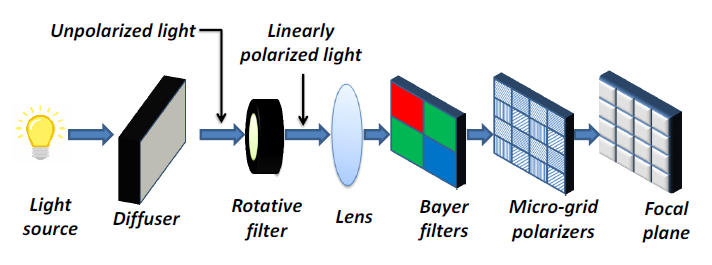
\includegraphics[width=8.5cm]{images/Figure_1.png}
    \caption{The experiment set up where only one super-pixel is represented.}
    \label{fig:my_label}
\end{figure}
of its robustness to outliers, the median value has been chosen and implemented for the experiments.

It is important to note that a color camera is used. To be free from the requirement of using a white light, the detected intensities and DoLP have to be classified per color channel, without mixing them. The color channel to which a super-pixel belongs to is given by its position \textit{j}.

At this point, an estimation of the light intensity $\hat{S}_0$, the degree of linear polarization $\hat{\rho}$ per color channel, and the angle of polarization $\hat{\alpha}_n$ at the $n^{th}$ position of the linear filter has been obtained. Therefore, the Stokes matrix can be built, as in Eq. (\textcolor{red}{21}),
\begin{equation}
   \hat{S} = \begin{bmatrix} \hat{S}_0 & 0 & 0 \\ 0 & \hat{S}_0\hat{\rho} & 0 \\ 0 & 0 & \hat{S}_0\hat{\rho} \end{bmatrix} \begin{bmatrix} 1 & ... & 1 \\ \cos(\hat{\alpha}_1) & ... & \cos(\hat{\alpha}_N) \\ \sin(\hat{\alpha}_1) & ... & \sin(\hat{\alpha}_N) \end{bmatrix} . 
\end{equation}
and its pseudo-inverse \textbf{$\hat{S}^+$} computed and used in Eq. (\textcolor{red}{10}) to calculate the $j^{th}$ super-pixel matrix that we will denote here by \textbf{$\hat{A}_j$}. It follows that, from \textbf{$\hat{A}_j$} each row allows to compute the parameters $(T_i, P_i, \theta_i)$ for each of the four pixels that compose the $j^{th}$ super-pixel.

\subsection{EXPERIMENTS}

Our experimental setup is composed of a Basler acA2440-75ucPOL camera with a Sony Polarsens IMX250MYR sensor of pixel size equal to $3.45\mu m$ or super-pixel size equal to $6.9\mu m$ , and a Fuji-film HF16XA-5M - F1.6/16mm lens. To compute an initial estimation of the AoLP and DoLP required by our calibration method, we have chosen a central region of 50 x 50 super-pixels determined according to Eq. (\textcolor{red}{13}). This region corresponds to incident light rays with a maximum angle of incidence of $0.625^{\circ}$ that is relatively small and will give a good initial estimation of the AoLP and DoLP.

The developed algorithm runs on a computer with Intel Core i7-10850H @ 2.7 GHz and 32 GB of RAM. The OS is Ubuntu 18.04 LTS 64 bits. The program runs in 7 seconds for 7 samples, and 8 seconds for 73 samples approximately. The experimental set-up model is shown in Fig. \textcolor{red}{3}. The uniform, unpolarized light source device is a Schott Fostec DCR III fiber optic illuminator, with a Schott ColdVision back light A08927. A 50mm linear glass polarizing filter is used (Edmund Optics Inc $\sharp 56-329$), mounted on a metric polarizer mount (Edmund Optics Inc $\sharp 43-787$). The linear polarizer filter is rotated by hand. Each position of the filter corresponds to a light sample, and for each sample ten acquisitions of the light are done and averaged to reduce the effects of the noise in the parameters estimation. The acquisitions are done
\begin{figure}
    \centering
    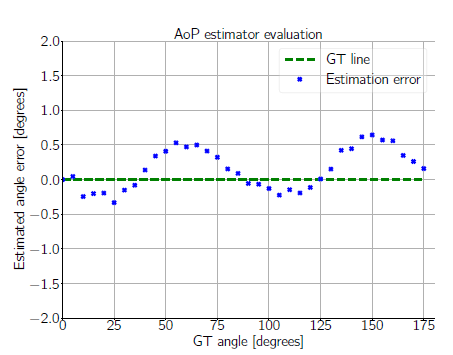
\includegraphics[width=8.5cm]{images/Figure_2.png}
    \caption{AoLP estimator evaluation. The maximum error is of $0.65^{\circ}$, and the RMSE is of $0.3316^{\circ}$ for all the range from [$0^{\circ}$; $180^{\circ}$]. The sine-like evolution is mainly due to the error in the polarizers orientations [\textcolor{green}{24}].}
    \label{fig:my_label}
\end{figure}
in a dark room to reduce the influence of the environment. Furthermore, the recommendations given in [\textcolor{green}{17}] have been followed. Particularly, the lens has been correctly focused at the light source, and the \textit{f}-number has been set higher than 2.8 for all the experiments. Finally, we have acquired several images with the camera in total darkness and verified that, with a 12-bit pixel count and an exposure time of 1s, the dark current can effectively be neglected as reported in [\textcolor{green}{17}].

The first experiment that we have done is to verify the quality of the estimated AoLP with the camera. To do so, different light samples with different AoLP have been used. The AoLP values are set by turning the polarization filter in front of the light source by steps of $5^{\circ}$, in the range $[5^{\circ}; 175^{\circ}]$. Thirty-six images of the source light samples are acquired with the camera, and from them the AoLP are calculated and compared to the true reference values given by the position of the polarization filter. For better visualization, only the deviations from the reference values are represented in Fig. \textcolor{green}{4}. In case the estimated AoLP values are the same as the reference values, an horizontal line at zero degree is obtained. However, in our case, the AoLP error curve exhibits a sine-like shape that is due to errors in the parameters of the camera. Indeed, it can be proven that a small error in the parameters of the camera due to imperfections will induce, in first order approximations, four error terms in the expression of the estimated AoLP. These error terms are functions of the sine and cosine of the true AoLP and they appear in the expressions of the computed Stokes components $S_1$ and $S_2$. Because of these additional components, and that the ratio of these two Stokes components is proportional to the tangent of the AoLP (Eq. (\textcolor{red}{1})), the error curve follows a sineand cosine rule. The detailed demonstration of this effect can be found in the supplementary material [\textcolor{green}{24}] (it is not included in the main paper since it is an auxiliary result of this work, and also due to space constraints). Nonetheless, by considering pixels around the center, and averaging several samples, the estimation error is reduced, such that the RMSE is $0.3316^{\circ}$, and the maximum error is $\pm 0.65^{\circ}$ in all the range. Hence, the experiment confirms that the camera can be used to provide reliable measurements of the AoLP of the ULP light. Additionally, it avoids the requirement of aligning the rotative.

\begin{figure}
    \centering
    \begin{tabular}{|c|c|c|c|}
        \hline
         &  
        $S_0$ & 
        $A_0LP$ & 
        $D_oLP$ \\
        \hline
        Uncalibrated & 3399.2 [65.475] & 59.983 [0.215]& 0.9863 [0.0041]\\
         \hline
         SP method & 3402.4 [10.723] & 60.035 [0.128] & 1.005 [0.004] \\
         \hline
         Our method & 3298.0 [10.402] & 59.701 [0.128] & 0.985 [0.004] \\
         \hline
    \end{tabular}
    \caption{TABLE 1}
    \label{fig:my_label}
\end{figure}

{\small
\bibliographystyle{IEEEtran}
\bibliography{references}
}

\end{document}

